\chapter{Stima di parametri}
In questo capitolo vedremo come usare i dati campionari per stimare una media,
una varianza o una proporzione della popolazione. Verranno discusse le stime puntuali
che sono stime a valore singolo del parametro. Verrà considerato poi l'errore standard di
queste stime. Inoltre considereremo gli intervallo di confidenza, che contengono il parametro
con un certo livello di confidenza.
\section{Statistica inferenziale}
La \textbf{statistica inferenziale} ha lo scopo di definire in modo non ambiguo e
quantitativo la plausibilità di un'inferenza.
\\ La plausibilità di un'inferenza dipende dal modo con cui è stato selezionato
il campione di n individui della popolazione.
La corretta metodologia di campionamento è la \textbf{scelta casuale}.
\\ Per la casualità dle campionamento utilizzo il calcolo delle probabilità.
\\ Quando parleremo di popolazione tratteremo sempre N molto grandi rispetto alla numerosità
del campione. 
\paragraph*{Popolazione} V.A. i.i.d. con la stessa distribuzione $\leftrightarrow$
legge F.
\\ Consideriamo il caso in cui F è nota a meno di qualche parametro incongito.
\paragraph*{Modello statistico parametrico} Famiglia di leggi note a meno di uno o
più parametri.
\begin{itemize}
    \item Caso discreto: $p(x; \Theta) \quad$ 
    Densità discreta $p(x;\Theta):\mathbb{P}_\Theta (X=x)$
    \item Caso continuo: densità $f(x; \Theta)$
\end{itemize}
\paragraph*{Attenzione} Non confondere le V.A. con le osservazioni
\begin{itemize}
    \item $X_1, ..., X_n \quad$ sono le v.a.
    \item $x_1, ..., X_n \quad$ sono le osservazioni
\end{itemize}
\paragraph*{Esempi di modelli statistici}
Esempi di modelli statistici sono:
\begin{itemize}
    \item Modello di Bernoulli
    \item Modello esponenziale
    \item Modello normale
\end{itemize}
Dato $(X_1, ..., X_n)$ campione casuale, si definisce \textbf{Statistica} una
funzione del campione, ossia una v.a. T della forma
\begin{equation*}
    T=f(X_1, ..., X_n)
\end{equation*}
\paragraph*{Esempi di statistiche}
\begin{itemize}
    \item $\bar{X}_n = \frac{X_1+...+X_n}{n} \quad$ Media campionaria (v.a.)
    \item $S^{2}_n = \frac{1}{n-1} \sum_{i=1}^n(X_i - \bar{X}_n)^2 \quad$ Varianza campionaria (v.a.)
\end{itemize}
\section{Statistica parametrica e Stimatori} 
Il primo obiettivo della statistica inferenziale è fornire una stima dei
parametri incogniti.   
\paragraph*{Stimatori} Uno \textbf{Stimatore} è una statistica il cui valore
dipende dal particolare campione che è stato estratto. Il valore dello stimatore,
\textbf{la Stima}, viene usato per predire il valore di un parametro della popolazione.
particolari statistiche che servono a stimare i parametri incogniti.
\paragraph*{Stimatori Puntuali} Sono valori singoli che speriamo siano prossimi
ai parametri stimati.
\paragraph*{Stimatori intervallari} Meglio noti come \textbf{Intervalli di confidenza},
in questo caso non rappresentano un singolo valore, ma un intervallo in cui ci
aspettiamo che il parametro rientri. Ci occupiamo anche di determinare quanta
confidenza associare a un dato intervallo, cioè quanto possiamo essere sicuro che il parametro
si trovi in questo intervallo.
\paragraph*{Definizione Stimatore Corretto} Uno \textbf{Stimatore} T si dice \textbf{Non Distorto o Corretto}
se:
\begin{equation*}
    \mathbb{E}_\Theta{T}: \mathbb{E}_\Theta(g(X_1, ..., X_n)) = \Theta
\end{equation*}
Dove $E_\Theta$ è il valore medio rispetto alla probabilità di $P_\Theta$.
\paragraph*{In parole povere} Uno stimatore il cui valore atteso è uguale al parametro
che si vuole stimare si dice \textbf{corretto} per quel parametro.
\paragraph*{$\bar{X}_n$ è lo stimatore non distorto di}
\begin{itemize}
    \item p in un modello di Bernoulli
    \item $\lambda$ in un modello di Poisson
    \item $\frac{1}{\lambda}$ in un modello esponenziale
    \item $\mu$ in un modello normale
\end{itemize}
\paragraph*{Osservazione} La proprietà di essere non distorto NON è stabile per
trasformazioni, ad esempio nel modlelo esponenziale $X_n$ è stimatore non distorto
di $\frac{1}{\lambda}$, ma si ha che $\frac{1}{\bar(X)_n}$ NON è uno stimatore non
distorto di $\lambda$.
\paragraph*{Stimatore consistente} Uno stimatore non distorto di $\Theta$ si dice
\textbf{Consistente} se, quando $n \rightarrow + \infty$
\begin{equation*}
    \text{Var}_\Theta (T) \rightarrow 0
\end{equation*}
Quando abbiamo un campione casuale estratto da una popolazione con media $\mu$
e varianza $\sigma^2$ finite si ha sempre che $\bar{X}_n$ \textbf{è uno stimatore consistente
di $\mu$}:
\begin{equation*}
    \text{Var}_\sigma(\bar{X}_n) = \frac{\sigma^2}{n} \rightarrow 0 \quad n \rightarrow + \infty
\end{equation*}
\\ Stimatore di $\Theta = g(X_1, ..., X_n) \rightarrow$ V.A.
\\ Stima di $\Theta: f(x_1, ..., X_n) \rightarrow$ Numero.
\\ Stima di $\mu$ per un campione casuale $X_1, ..., X_n$ di cui osserviamo
$x_1, ..., x_n$.
\begin{equation*}
    \hat{\mu} = \bar{x}_n = \frac{x_1+...+x_n}{n}
\end{equation*}
\section{Errore standard}
Supponiamo di considerare un campione casuale con media $\mu$ incognita
e varianza $\sigma$ nota:
\begin{equation*}
    \text{Var}\bar{X}_n= \frac{\sigma^2}{n}
\end{equation*}
\begin{equation*}
    \text{SD}(\bar{X}_n) = \frac{\sigma}{\sqrt{n}} \quad \text{deviazione standard SD}
\end{equation*}
Se si pensa $\bar{X}_n$ come stimatore di $\mu$, SD$(\bar{X}_n)$ prende il nome Di
\textbf{errore standard}, esso rappresenta l'errore commesso stimando $\mu$ con $\bar{X}_n$.
\\ Ora consideriamo un modello statistico con \textbf{varianza incognita}.
\\ In statistica descrittiva: siano n osservazioni $(x_1, ..., x_n)$;
\begin{equation*}
    s^{2}_n=\frac{1}{n-1}\sum_{k=1}^n(x_k-\bar{x}_n)^2
\end{equation*}
\'E sensato introdurre in un modello statistico con varianza $\sigma^2$ incognita lo
stimatore
\begin{equation*}
    S^{2}_n=\frac{1}{n-1}\sum_{k=1}^n(X_k-\bar{X}_n)^2
\end{equation*}
Se nel modello statistico con varianza $\sigma^2$ incognita \textbf{la media è nota}, si ha che
lo stimatore:
\begin{equation*}
    \bar{S}^{2}_n = \frac{1}{n}\sum_{i=1}^n(X_u - \mu)^2
\end{equation*}
è uno stimatore corretto di $\sigma^2$.
\section{Chi quadrato}
\subsection*{Distribuzione delle statistiche campionarie}
\paragraph*{Campione normale}
$X_1, ..., X_n$ campione casuale $\mathcal{N}(\mu, \sigma^2)$
\begin{equation*}
    \bar{X}_n \sim \mathcal{N}(\mu, \frac{\sigma^2}{n})
\end{equation*}
Standardizzando otteniamo
\begin{equation*}
    \frac{\bar{X}_n-\mu}{\frac{\sigma}{\sqrt{n}}} \sim \mathcal{N}(0,1)
\end{equation*}
Per caratterizzare la legge di $S_{n}^2$ e di $\bar{S}_{n}^2$ dobbiamo
introdurre una nuova distribuzione continua
\begin{equation*}
    \chi^2(n)
\end{equation*}
Si dice legge \textbf{chi quadrato con n gradi di libertà} la legge di una v.a.
\begin{equation*}
    Y = \sum_{i=1}^n Z_{i}^2 \,, \quad z_1, ..., z_n \quad \text{i.i.d.}\quad \mathcal{N}(0,1)
\end{equation*}
%Video Lezione 10 T1 minuto 32:29 - https://elearning.unimib.it/mod/kalvidres/view.php?id=926811
Dove Y è una v.a. $\geq 0$ con densità $f_r(t) = c_n t^{\frac{n}{2}-1} e^{-\frac{t}{2}} 
\qquad \text{per} \quad t>0$
\\ Si ha $\mathbb{E}(Y) = n$ e $\text{Var}(Y)=2n$
\\ Per $n = 2$ è la legge $\text{exp}(\frac{1}{2})$
\\ Per n grande vale l'approssimazione della legge $\chi^2(n)$ con una
$\mathcal{N}(n,2n)$
\paragraph*{Proposizione} Sia $(X_1, ..., X_n)$ campione casuale estratto
da una popolazione $\mathcal{N}(\mu, \sigma^2)$.
\begin{enumerate}
    \item $\sum_{i=1}^n(\frac{X_i-\mu}{\sigma})^2 \sim \chi^2(n)$
    \item $\sum_{i=1}^n(\frac{X_i-\bar{X}_n}{\sigma}) \sim \chi^2(n-1)$
    \item se $S_{n}^2 = \frac{1}{n-1}\sum_{i=1}^n(X_i - \bar{X}_n)^2$
    \\ $(n-1)\frac{S_{n}^2}{\sigma^2} \sim \chi^2(n-1)$
    \item $S_{n}^2$ e $\bar{X}_n$ sono indipendenti
\end{enumerate}
Riassumendo $\chi^2$ ci serve per la distribuzione della legge delle varianze campionarie
\section{Distribuzione t di student}
\paragraph*{Definizione Wikipedia} 
Nella teoria delle probabilità la distribuzione di Student, o t di Student, 
è una distribuzione di probabilità continua che governa il rapporto tra due variabili aleatorie, 
la prima con distribuzione normale e la seconda, al quadrato, segue una distribuzione chi quadrato.
\\ Questa distribuzione interviene nella stima della media di una popolazione che segue la distribuzione normale, 
e viene utilizzata negli omonimi test t di Student per la significatività e per ogni intervallo 
di confidenza della differenza tra due medie. 
\paragraph*{Definizione matematica}Si dice legge di \textbf{t di student con n gradi di libertà} la legge di una v.a.
\begin{equation*}
    T = \frac{z}{\sqrt{\frac{Y}{n}}}
\end{equation*}
\begin{equation*}
    z \sim \mathcal{N}(0,1)
\end{equation*}
\begin{equation*}
    Y \sim \chi^2(n)
\end{equation*}
Z e Y sono indipendenti.
\begin{equation*}
    \mathbb{E}(T)=0 \quad \text{Var}[T] = 1
\end{equation*}
T è una v.a. continua con densità
\begin{equation*}
    f_T(t) = c_n(1+\frac{t^2}{n})^{\frac{-(n+1)}{2}}
\end{equation*}
$c_n$ è una costante che fa risultare l'integrale della $f = 1$.
\paragraph*{Proposizione} Sia $X_1, ..., X_n$ un campione casuale estratto da
una popolazione $\mathcal{N}(\mu, \sigma^2)$. Allora
\begin{equation*}
    \frac{\bar{X}_n-\mu}{\sqrt{\frac{s^2_{n}}{n}}} \sim t(n-1)
\end{equation*}
\section{Parte pratica}
Cosa dovremo saper calcolare di queste variabili aleatorie? I loro percentili.
\\ X v.a.
\\ $P(X\leq q_\alpha) = \alpha$ Fissato $\alpha$, trovare $q_\alpha$.
\\ $q_\alpha$ = $\alpha$ - esimo quantile o $100\alpha$ - percentile di X.
\begin{itemize}
    \item $Z \sim \mathcal{N}(0,1) \qquad z_\alpha$ t.c. $\mathbb{P}(Z>z_\alpha) = \alpha$
    \item $T \sim t(n) \qquad t_{\alpha, n}$ t.c. $\mathbb{P}(T>t_{\alpha, n}) = \alpha$
    \item $Y \sim \chi^2{n} \qquad \chi^2_{\alpha, n}$ t.c. $\mathbb{P}(Y>\chi^2_{\alpha,n}) = \alpha$
    \item $z_\alpha$, $t_{n, \alpha}$, $\chi^2_{m, \alpha} 
    \qquad 100(1-\alpha) \text{percentili} \quad (\text{di}\quad Z, T, Y)$
\end{itemize}
\begin{equation*}
    Z \sim \mathcal{N}(0,1) \qquad \alpha \quad \text{definito da}
\end{equation*}
\begin{gather*}
    P(Z>z_\alpha) = \alpha \\
    P(Z\leq Z_\alpha) = 1-\alpha \\
    z_\alpha = 100(1-\alpha) \qquad \text{percentili di Z}\\
    z_\alpha = \Phi^{-1}{1-\alpha} \\
    P(Y > X^2_{\alpha, n}) = \alpha
\end{gather*}
La simmetria di T student è la stessa della normale.
\\ Mentre per la $\chi^2$ non ci sono simmetrie.
\begin{center}
    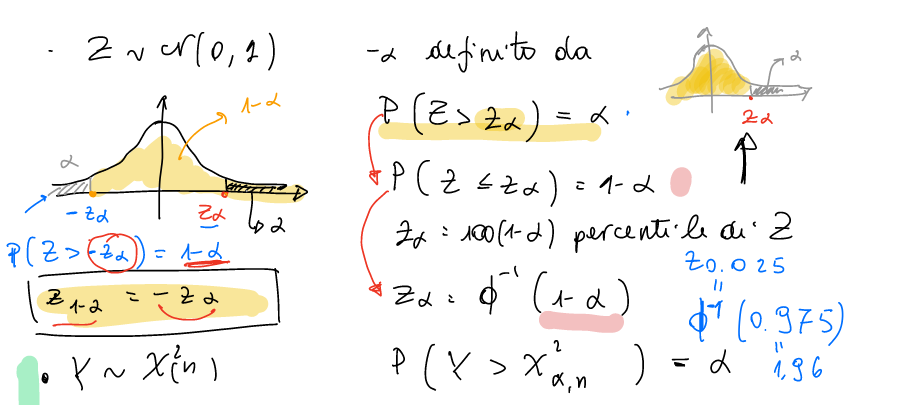
\includegraphics[width=120mm,scale=0.5]{Simmetria t di student.png}
\end{center}

\section{Stima per intervalli - Intervalli di confidenza}
Stima per intervalli della media - campione normale $\mathcal{N}(\mu, \sigma^2)$, con
$\sigma^2$ nota.

La qualità dlela stima dipende Da
\begin{itemize}
    \item Livelli di confidenza: maggiore è il livello, più è affidabile è la stima
    \item Ampiezza dell'intervallo = $2E$: più è piccolo, più è precisa la stima
\end{itemize}
\begin{equation*}
    E=Z_{\frac{\alpha}{2}}\frac{\sigma}{\sqrt{n}}
\end{equation*}
E crece se $\alpha$ diminuisce (ossia se la confidenza aumenta) fissati n e $\sigma$
E diminuisce al crescere di n (come $\frac{1}{\sqrt[]{n}})$
\subsection*{Estremi Inferiori e Superiori di Confidenza Per la media di una popolazione normale con varianza nota.}
Per la media di una popolazione normale con varianza nota.
\\ Determinare se la media di una popolazione è maggiore o minore di un certo
valore.
\\ Useremo ancora $\frac{\bar{X}_n - \mu}{\frac{\sigma}{\sqrt[]{n}}} = 
\sqrt[]{n} \frac{\bar{X}_n - \mu}{\sigma} \sim \mathcal{N}(0,1)$ 
\\ Confidenza: $100(1-\alpha) \%$
\begin{gather*}
    \mathbb{P}(\frac{(\bar{X}_n - \mu)}{\frac{\sigma}{\sqrt[]{n}}} < z_\alpha) 
    = 1 - \alpha \\
    \mathbb{P}(\mu > \bar{X}_n - z_\alpha \frac{\sigma}{\sqrt[]{n}} = \ - \alpha)
\end{gather*}
Un estremo inferiore di confidenza al $100(1-\alpha)\%$ per la media di una
popolazione normale con varianza nota è dato da
\begin{equation*}
    \bar{X}_n - z_\alpha \frac{\sigma}{\sqrt[]{n}}
\end{equation*}
La sua realizzazione (dai dati campionari) è:
\begin{equation*}
    \bar{x}_n - z_\alpha\frac{\sigma}{\sqrt[]{n}}
\end{equation*}
\subsection*{Intervalli di confidenza per la media di una popolazione normale con varianza incognita}
Completare -----------------------------------
Possiamo dire:
\begin{itemize}
    \item Confidenza maggiore $\rightarrow$ E aumenta (a parità del campione), però la
    stima è più affidabile
    \item Estremo inferiore di confidenza al $100(1-\alpha) \%$
    \item Estremo superiore di confidenza al $100(1-\alpha) \%$
\end{itemize}
\subsection*{Intervalli di confidenza per la varianza di una popolazione normale}

%Verifica di Ipotesi%
